%%%%%%%%%%%%%%%%%%%%%%%%%%%%%%%%%%%%%%%%%
% a0poster Portrait Poster
% LaTeX Template
% Version 1.0 (22/06/13)
%
% The a0poster class was created by:
% Gerlinde Kettl and Matthias Weiser (tex@kettl.de)
%
% This template has been downloaded from:
% http://www.LaTeXTemplates.com
%
% License:
% CC BY-NC-SA 3.0 (http://creativecommons.org/licenses/by-nc-sa/3.0/)
%
%%%%%%%%%%%%%%%%%%%%%%%%%%%%%%%%%%%%%%%%%

%----------------------------------------------------------------------------------------
%	PACKAGES AND OTHER DOCUMENT CONFIGURATIONS
%----------------------------------------------------------------------------------------

\documentclass[a0,portrait]{a0poster}

\usepackage{multicol} % This is so we can have multiple columns of text side-by-side
\columnsep=100pt % This is the amount of white space between the columns in the poster
\columnseprule=3pt % This is the thickness of the black line between the columns in the poster

\usepackage[svgnames]{xcolor} % Specify colors by their 'svgnames', for a full list of all colors available see here: http://www.latextemplates.com/svgnames-colors

\usepackage{times} % Use the times font
%\usepackage{palatino} % Uncomment to use the Palatino font

\usepackage{graphicx} % Required for including images
\graphicspath{{figures/}} % Location of the graphics files
\usepackage{booktabs} % Top and bottom rules for table
\usepackage[font=small,labelfont=bf]{caption} % Required for specifying captions to tables and figures
\usepackage{amsfonts, amsmath, amsthm, amssymb} % For math fonts, symbols and environments
\usepackage{wrapfig} % Allows wrapping text around tables and figures
\usepackage{bbm}
\usepackage{smartdiagram}

\begin{document}

%----------------------------------------------------------------------------------------
%	POSTER HEADER
%----------------------------------------------------------------------------------------

% The header is divided into two boxes:
% The first is 75% wide and houses the title, subtitle, names, university/organization and contact information
% The second is 25% wide and houses a logo for your university/organization or a photo of you
% The widths of these boxes can be easily edited to accommodate your content as you see fit

\begin{minipage}[b]{0.75\linewidth}
\veryHuge \color{NavyBlue} \textbf{Towards Perceptual Soundscape Characterization Using\- Event Detection Algorithms} \color{Black}\\ % Title
\Huge\textit{}\\[2cm] % Subtitle
\huge \textbf{F\'elix Gontier, Pierre Aumond, Mathieu Lagrange,\\ Catherine Lavandier, Jean-Francois Petiot}\\[0.5cm] % Author(s)
\huge LS2N, CNRS, \'Ecole Centrale de Nantes\\[0.4cm] % University/organization
\end{minipage}
%
\begin{minipage}[b]{0.25\linewidth}

\includegraphics[width=20cm]{logoLs2n.jpg}\\
\end{minipage}

\vspace{1cm} % A bit of extra whitespace between the header and poster content

%----------------------------------------------------------------------------------------

\begin{multicols}{2} % This is how many columns your poster will be broken into, a portrait poster is generally split into 2 columns

%----------------------------------------------------------------------------------------
%	ABSTRACT
%----------------------------------------------------------------------------------------

\color{Navy} % Navy color for the abstract

\begin{abstract}

Assessing properties about specific sound sources is important to  characterize better the perception of urban sound environments. In order to produce perceptually motivated noise maps, we argue that it is possible to consider the data produced by acoustic sensor networks to gather information about sources of interest and predict their perceptual attributes.

To validate this important assumption, this paper reports on a perceptual test on simulated sound scenes for which both perceptual and acoustic source properties are known. Results show that it is indeed feasible to predict perceptual source-specific quantities of interest from recordings, leading to the introduction of two predictors of perceptual judgments from acoustic data. The use of those predictors in the new task of automatic soundscape characterization is finally discussed.

\end{abstract}



%----------------------------------------------------------------------------------------
%	INTRODUCTION
%----------------------------------------------------------------------------------------

\color{SaddleBrown} % SaddleBrown color for the introduction

\section*{Perceptual soundscape characterization}

The deterioration of \textbf{sound quality in urban} environments is an \textbf{increasing concern}. In this context, the perception of a soundscape by city dwellers is an essential part of its characterization. Perceptual spaces are constructed that associate the soundscape to subjective parameters. Specifically, the dimension of pleasantness has already been extensively studied through perceptual experiments~\cite{aumond2017}. It is consistently modeled as a function of both the sound scene's overall characteristics (loudness) and source-specific contents, typically the time of presence:
\begin{equation}
P = aL + \sum_s b_sT_{s,p} + c
\end{equation}

Although previous studies focus on subjective data, the resulting models hint at the possibility of predicting pleasantness from acoustical indicators.


\vspace{1cm}


\hyphenpenalty10000
\exhyphenpenalty10000

\smartdiagramset{
				 uniform color list=white!60!gray for 3 items,
				 back arrow disabled=true,
				 module minimum width=10cm,
				 }
				 \smartdiagram[flow diagram:horizontal]{Event detection, perceived time of presence, Pleasantness prediction}
%	}


The corresponding task could thus be formulated as a three-level processing chain. At the first level event detection and source separation algorithms are used to determine the contents of the scene in terms of acoustical properties and source activity. The second level is the estimation of perceived time of presence for each source, for which the relevant time scale is longer. Finally, pleasantness is predicted using the available perceptual models.

%----------------------------------------------------------------------------------------
%	OBJECTIVES
%----------------------------------------------------------------------------------------

\begin{center}\vspace{1cm}
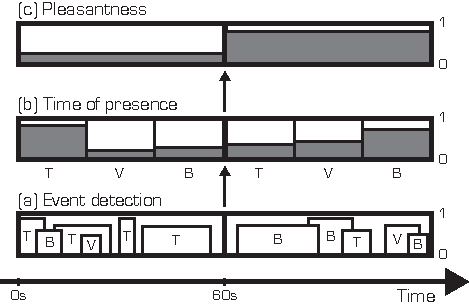
\includegraphics[width=0.65\linewidth]{block.pdf}
\captionof{figure}{ \color{RoyalBlue} The three suggested levels of metrics to predict soundscape pleasantness. Traffic, voices and birds are considered as having the most influence on pleasantness in past studies.}
\end{center}

\color{DarkSlateGray} % DarkSlateGray color for the rest of the content



\section*{Contributions}

The main contributions of this work are as follows:
\begin{itemize}
\item A \textbf{perceptual validation} of the feasibility of estimating the perceived source activity from acoustical data,
\item The proposition of source-specific \textbf{physical indicators} in order to achieve this prediction.
\end{itemize}

\section*{Perceptual validation}
 \begin{minipage}[c]{.48\linewidth}
A perceptual experiment is conducted to ensure that the prediction of source-specific perceived time of presence from acoustical data is possible. A corpus of 9 simulated scenes from~\cite{gloaguen2017} is studied in which 5 different sources are active (traffic, birds, horns, voices, footsteps). The questions include 4 general perceptual dimensions and the source-specific time of presence and sound level. 28 students from \'Ecole Centrale de Nantes performed the test. The study generates a perceptual space coherent with the litterature~\cite{axelsson2010}, indicating the relevance of the considered corpus.
\end{minipage}
\hfill
 \begin{minipage}[c]{.48\linewidth}
\begin{center}\vspace{1cm}
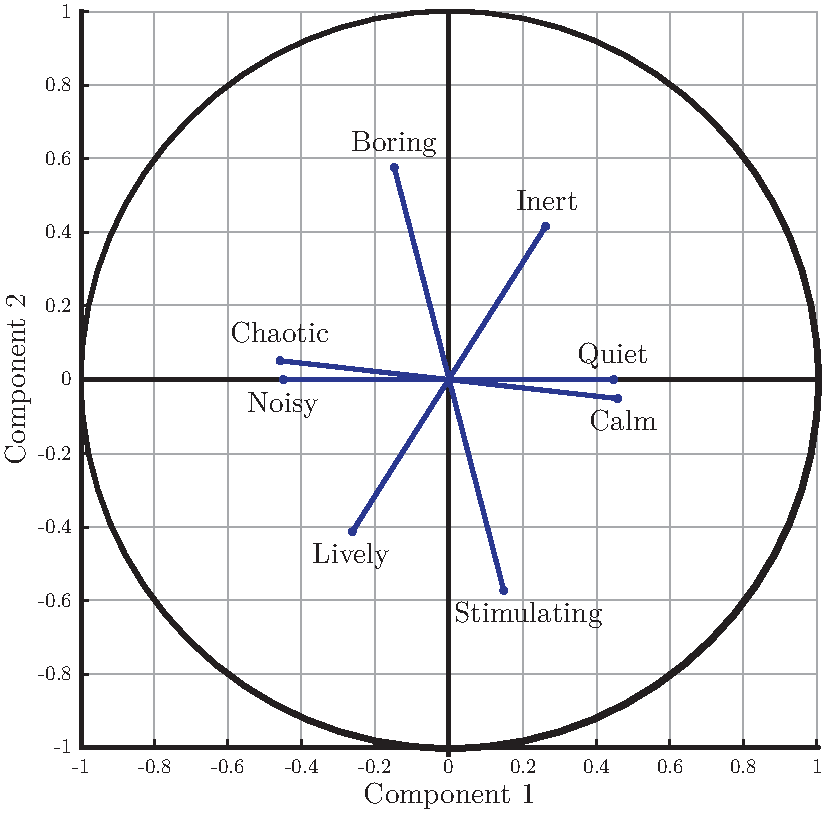
\includegraphics[width=.8\linewidth]{pca.pdf}
\captionof{figure}{ \color{RoyalBlue} Perceptual space of the study.}
\end{center}
\end{minipage}
\vspace{1cm}

\section*{Physical indicators}


Global sound levels $L_{50}$, $L_{A50}$ and $L_{50, 1kHz}$ are considered as they represent well the scene's perceived overall loudness~\cite{aumond2017}. As simulated scenes are studied the ground truth source contributions are available. The time of presence and an emergence metric ($L_{10, source}-L_{90, global}$) are computed per source from the separated audio file.

To account for masking effects, two additional indicators are proposed that respectively consider overall and frequency-wise source emergence over time frames to approximate the corresponding perceived time of presence:

\begin{align}
T_s(\alpha) &= \frac{1}{N_t}\sum_{t = 1}^{N_t}\mathbbm{1}_{L_s(t) - L_b(t)>\alpha} \\
T_s(\alpha, \beta) &= \frac{1}{N_t}\sum_{t = 1}^{N_t}\mathbbm{1}\left[ \frac{\sum_{f = 1}^{N_f}\Delta_s(t, f)\mathbbm{1}_{\Delta_s(t, f)>\alpha}}{\sum_{f = 1}^{N_f}\mathbbm{1}_{\Delta_s(t, f)>\alpha}}>\beta \right], \Delta_s(t, f) = L_s(t, f) - L_b(t, f)
\end{align}

The optimization of parameters $\alpha$ and $\beta$ is done via grid search on the considered corpus due to the lack of other available perceptual data.

\section*{Results}

Globally computed sound levels represent very well the perceived overall loudness ($r>0.95$, $p<0.01$). The ground truth source-specific time of presence and emergence achieve good results for most sources. However they fail to describe traffic activity, which is present in the background of most scenes but can be masked by more emergent sources. The use of metrics considering each source independantly from one another is thus not sufficient.

The proposed binary masking models solve this problem as an active source can be considered unheard in the mix. They correlate consistently well with the perceived time of presence, and successfully discriminate between sources such as traffic and birds, which are commonly correlated in real-life conditions.

\begin{center}\vspace{1cm}
\label{table:pearsonc}
%\resizebox{\columnwidth}{!}{
\begin{tabular}{ l | c c c c c c c c c c }
\hline
	Phys./Perc. & $L_{T,p}$ & $T_{T,p}$ & $L_{B,p}$ & $T_{B,p}$ & $L_{H,p}$ & $T_{H,p}$ & $L_{V,p}$ & $T_{V,p}$ & $L_{F,p}$ & $T_{F,p}$ \\ \hline
	$T_T$ & NS & NS & NS & NS & NS & NS & NS & NS & NS & NS \\
	$L_T$ & NS & NS & NS & NS & NS & NS & NS & NS & NS & NS \\ \hline
	$T_B$ & 0.71* & 0.75* & NS & NS & NS & NS & NS & NS & NS & NS \\
	$L_B$ & -0.84** & -0.83** & 0.91** & 0.82** & NS & NS & NS & NS & NS & NS \\ \hline
	$T_H$ & NS & NS & NS & NS & NS & 0.84** & NS & NS & NS & NS \\
	$L_H$ & NS & NS & NS & NS & 0.98** & 0.78* & NS & NS & NS & NS \\ \hline
	$T_V$ & NS & NS & NS & NS & NS & NS & NS & NS & NS & NS \\
	$L_V$ & NS & NS & NS & NS & NS & NS & 0.84** & 0.88** & NS & NS \\ \hline
	$T_F$ & NS & NS & NS & NS & NS & NS & NS & NS & 0.9** & 0.68* \\
	$L_F$ & NS & NS & NS & NS & NS & NS & -0.69* & -0.78* & 0.92** & NS \\ \hline
	$T_T(\alpha)$ & 0.90** & 0.94** & NS & NS & NS & NS & NS & NS & NS & NS \\
	$T_T(\alpha, \beta)$ & 0.88** & 0.92** & NS & NS & NS & NS & NS & NS & NS & NS \\ \hline
	$T_B(\alpha)$ & NS & NS & 0.95** & 0.97** & NS & NS & NS & NS & NS & NS \\
	$T_B(\alpha, \beta)$ & NS & NS & 0.95** & 0.97** & NS & NS & NS & NS & NS & NS \\ \hline
	$T_H(\alpha)$ & NS & NS & NS & NS & NS & 0.83** & NS & NS & NS & NS \\
	$T_H(\alpha, \beta)$ & NS & NS & NS & NS & 0.73* & 0.88** & NS & NS & NS & NS \\ \hline
	$T_V(\alpha)$ & NS & NS & NS & NS & NS & NS & 0.79* & 0.83** & NS & NS \\
	$T_V(\alpha, \beta)$ & NS & NS & NS & NS & NS & NS & 0.75* & 0.79* & NS & NS \\ \hline
	$T_F(\alpha)$ & NS & NS & NS & NS & NS & NS & NS & -0.71* & 0.87** & NS \\
	$T_F(\alpha, \beta)$ & NS & NS & NS & NS & NS & NS & NS & NS & 0.90** & 0.70* \\ \hline
\end{tabular}
%}
\captionof{table}{ \color{RoyalBlue} Pearson correlation coefficients between perceptual parameters and physical indicators at the scene level (n=9). *: $p<0.05$, **: $p<0.01$, non-significant correlations ($p>0.05$) are noted NS.}
\end{center}\vspace{1cm}



%----------------------------------------------------------------------------------------
%	CONCLUSIONS
%----------------------------------------------------------------------------------------

\color{SaddleBrown} % SaddleBrown color for the conclusions to make them stand out

\section*{Conclusions}

A binary masking model is proposed that relies on the time of presence and emergence of sources. It is shown to correlate well with perceptual time of presence equivalents. Pleasantness prediction in urban soundscapes task can thus be formulated as a detection and classification task. Furthermore, low time resolutions compared to traditional event detection algorithms are sufficient to capture the information at the perceptual level.



\color{DarkSlateGray} % Set the color back to DarkSlateGray for the rest of the content

%----------------------------------------------------------------------------------------
%	FORTHCOMING RESEARCH
%----------------------------------------------------------------------------------------

\section*{Forthcoming Research}

Our future work includes conducting a refined perceptual experiment with the following considerations:
\begin{itemize}
\item A richer corpus should be studied, that is not limited to real-life conditions but includes more diverse source contributions,
\item State-of-the-art masking models should be compared to the proposed indicators,
\item Quantities of interest should be predicted from recordings through detection or source separation algorithms.
\end{itemize}
The final objective is the formulation of a complete experimental protocol for pleasantness prediction with respect to the experimental results.




 %----------------------------------------------------------------------------------------
%	REFERENCES
%----------------------------------------------------------------------------------------

\nocite{*} % Print all references regardless of whether they were cited in the poster or not
\bibliographystyle{plain} % Plain referencing style
\bibliography{sample} % Use the example bibliography file sample.bib

%----------------------------------------------------------------------------------------
%	ACKNOWLEDGEMENTS
%----------------------------------------------------------------------------------------

\section*{Acknowledgements}

The authors would like to acknowledge support for this project from ANR project Cense (grant ANR-16-CE22-0012).
%----------------------------------------------------------------------------------------

\end{multicols}
\end{document}
